\subsection{Серверное ПО и лицензирование}

Для работы программных пакетов, представленных в задании на разработку, необходима ОС
семейства Windows. Также, необходима ОС, позволяющая многопользовательскую работу, то
есть Windows Server. Актуальная на момент разработки версия — Windows Server 2019. У
данной версии есть три варианта: Essentials, Standart и Datacenter.
\cite{ref:win_srv_overview}\cite{ref:win_srv_comp}.

\begin{table}[h]
    \centering
    \caption{Сравнение редакций Windows Server 2019}
    \label{tab:win_srv_comp}
    \begin{tabu}to \linewidth{X[1,c,m]X[1,c,m]X[1,c,m]X[1,c,m]}
        \toprule
        Редакция & Essentials & Standart & Datacenter \\
        \midrule
        Лицензирование & На сервер & На ядро + CAL & На ядро + CAL \\
        Виртуализация & Да & Да; 2~виртуальные
        машины и один узел Hyper-V на лицензию & Да; неограниченное количество
        виртуальных машин и один узел Hyper-V на лицензию. \\
        Защищенные виртуальные машины & Нет & Нет & Да \\
        Программные сетевые интерфейсы & Нет & Нет & Да \\
        Программное хранилище данных & Нет & Нет & Да \\
        \bottomrule
    \end{tabu}
\end{table}

\begin{enumerate}
    \item Datacenter ‒ предназначен для развёртывания в облачных средах и в центрах по
        обработке данных при высоком уровне виртуализации. Лицензия приобретается по
        принципу: одна лицензия \say{на ядро} (core-based);
    \item Standard ‒ ориентирована для использования в среде с минимальными уровнями
        виртуализации, а также в физической среде. Лицензирование производится так же,
        как и в случае с \say{Datacenter};
    \item Essentials ‒ редакция, ориентированная на малый бизнес, с ограничением на
        количество клиентов — допускается не более 50 устройств и максимум 25
        пользователей. Данная редакция получает лицензию по методу server-based:
        один физический сервер – одна лицензия (на каждый дополнительный сервер
        необходимо приобретать новую лицензию).
\end{enumerate}

Подробное сравнение этих вариантов приводится в таблице~\ref{tab:win_srv_comp}.
Также стоит отметить, что для многопользовательской работы в редакциях Standart и
Datacenter необходимо покупать дополнительные лицензии для каждого клиента. Такие
лицензии называются Client Activation License (CAL).

Исходя из этих ограничений, можно выбрать редакцию Essentials для разрабатываемого
проекта. Ограничения касаются в основном функций виртуализации, которые в данном проекте
не используются.

\subsection{Выбор используемого протокола}

Для разработки необходимо выбрать способ удаленного доступа, который будет
использоваться в системе. Так как выбор зависит от серверной ОС, выбор оптимального
варианта связан с доступными на Windows протоколами.

Основной протокол, используемый в Windows — RDP (Remote Desktop Protocol). Клиент RDP
доступен во всех редакциях Windows, начиная с Windows XP, что позволяет использовать
любой компьютер кафедры в качестве тонкого клиента (см. рисунок \ref{pic:mstsc_xp}).
Однако, RDP-клиенты существуют для многих платформ, в том числе для Linux.

Актуальные версии протокола RDP:
\begin{itemize}
    \item Версия 6.0 установлена в Windows Vista и включила поддержку программ
        удаленного взаимодействия, приложениям Windows Presentation Foundation,
        поддержку нескольких мониторов и поддержку большого рабочего стола. Эта версия
        доступна для Windows XP с пакетом обновления (SP2), Windows Server 2003 SP1 /
        SP2 (выпуски x86 и x64) и Windows XP Professional x64 Edition. Microsoft Remote
        Desktop Connection для Macintosh OS X также доступен с поддержкой Intel и
        PowerPC Mac OS версии 10.4.9 и выше.
        
    \item Версия 6.1 была выпущена в феврале 2007 и включена в Windows Server 2008, и в
        пакет обновления Windows Vista SP1 и Windows XP SP3.  В дополнение к изменениям,
        связанным с улучшенным доступом к консоли, эта версия включает новые
        функциональные возможности, появившиеся в Windows Server 2008, такие как
        Terminal Services Easy Print driver (новая клиентская система перенаправления
        принтера, которая позволяет выполнять локальную печать из приложений,
        выполняющихся на сервере, не устанавливая драйвер печати на сервере).
    \item Версия 7 (вышла в составе Windows 7, поддерживается в Windows XP). Особенности
        этой версии:
    \begin{itemize}
        \item Поддержка аутентификации сетевого уровня (NLA), что снижает риск успешной
            атаки типа отказ в обслуживании (DoS);
        \item Увеличение производительности ядра RDP;
        \item Поддержка технологии Windows Aero (Aero over Remote Desktop);
        \item Поддержка технологий Direct2D и Direct3D 10.1 в приложениях;
        \item Полноценная поддержка мультидисплейных конфигураций;
        \item Улучшения в работе с мультимедиа;
        \item Поддержка технологии Media Foundation;
        \item Поддержка технологии DirectShow;
        \item Снижена длительность задержки при воспроизведении аудио.
    \end{itemize}

    \item Версия 7.1 (вышла в составе Windows 7 SP1);
    \item Версия 8.0 (вышла в составе Windows 8, с октября 2012 года доступна как пакет
        обновления для Windows 7 SP1 и Windows Server 2008);
    \item Версия 8.1 (вышла в составе Windows 8.1, с ноября 2013 года доступна как пакет
        обновления для Windows 7 SP1 и Windows Server 2008 R2);
    \item Версия 10 (Вышла в составе Windows 10, с 29 июля 2015 года. Последней версией
        является 10.0.16299.15, входящей в состав Windows 10 1809. Десятая версия
        включает в себя ряд новых функций, например, масштабирование AutoSize (полезно
        для клиентов HiDPI). Улучшен алгоритм сжатия графики с использованием H.264/AVC.
\end{itemize}

Используемая версия протокола RDP — 10, последняя на данный момент, т.к. используется
актуальная версия Windows Server.

\subsection{Клиентское ПО}

В качестве клиентской ОС выбран стандартный для Raspberry Pi дистрибутив Linux Raspbian,
основанный на Debian \cite{ref:raspbian}.
Дистрибутив поддерживается Raspberry Pi Foundation и рекомендован к установке.
К его преимуществам можно отнести открытый исходный код, простоту установки и удобство 
настройки. 
Актуальной на момент разработки была версия Buster, вышедшая в феврале 2020 года.

При загрузке ОС пользователь будет попадать в менеджер окон Openbox. Он настроен на
автоматический запуск RDP-клиента, также в случае необходимости (например, для
устранения проблем с сетевым подключением) его можно будет настроить для работы в режиме
обычного ПК, то есть как \say{толстый клиент}.

Для RDP-клиента использовано ПО FreeRDP, актуальной на момент разработки версии 2.0.0
\cite{ref:freerdp}. Данный программный продукт позволяет осуществлять подключение к
RDP-серверам любой версии, просто и гибко настраивается для получения оптимальной
производительности.  Так как исходный код открыт, есть возможность скомпилировать
бинарный файл для нужной архитектуры (в рассматриваемом проекте используется архитектура
ARM).

Так как FreeRDP не имеет графического интерфейса, для запуска будет использован скрипт,
выполняющийся при загрузке системы и позволяющий сразу подключиться к серверу. 

\begin{figure}[h]
    \center
    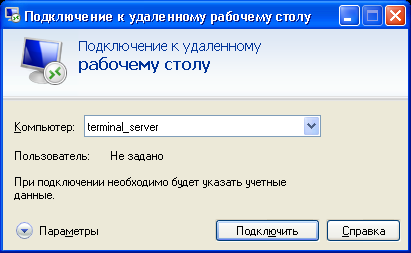
\includegraphics[height=8cm]{mstsc_xp}
    \caption{Окно RDP-клиента, встроенного в Windows XP}
    \label{pic:mstsc_xp}
\end{figure}

\begin{figure}[h]
    \center
    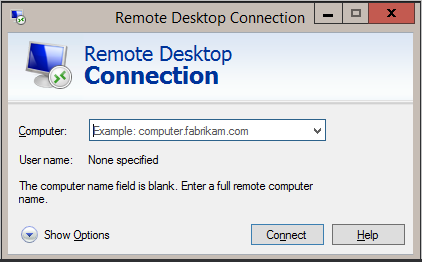
\includegraphics[height=8cm]{mstsc_10}
    \caption{Окно RDP-клиента, встроенного в Windows 10}
    \label{pic:mstsc_10}
\end{figure}

Также при необходимости подключения Windows-клиентов может быть использован встроенный в
систему RDP-клиент (см. рисунки~\ref{pic:mstsc_xp},~\ref{pic:mstsc_10}). Это может быть
полезным, в том числе, для подключения личных ноутбуков студентов.
